\subsection{Overview}
The defining characteristic of the model is the modeling of real rather than synthetic cohorts, all of whom 
are followed at the individual level. This allows for more heterogeneity in behavior than would be allowed 
by a cell-based approach. Also, since the PSID interviews both respondent and spouse, we can link records to 
calculate household-level outcomes, which depend on the responses of both spouses. 

The model has three core components: 

\begin{itemize}
\item The replenishing cohort module predicts the economic and health outcomes of new cohorts of 25/26 year-olds. This 
module takes in data from the Panel Survey of Income Dynamics (PSID) and trends calculated from other sources. It 
allows us to �generate� cohorts as the simulation proceeds, so that we can measure outcomes for the age 25+ 
population in any given year. 
\item The transition module calculates the probabilities of transiting across various health states and financial 
outcomes. The module takes as inputs risk factors such as smoking, weight, age and education, along with lagged 
health and financial states. This allows for a great deal of heterogeneity and fairly general feedback effects. 
The transition probabilities are estimated from the longitudinal data in the PSID. 
\item The policy outcomes module aggregates projections of individual-level outcomes into policy outcomes such as 
taxes, medical care costs, and disability benefits. This component takes account of public 
and private program rules to the extent allowed by the available outcomes.  
\end{itemize}

\begin{figure}[h]
\centering
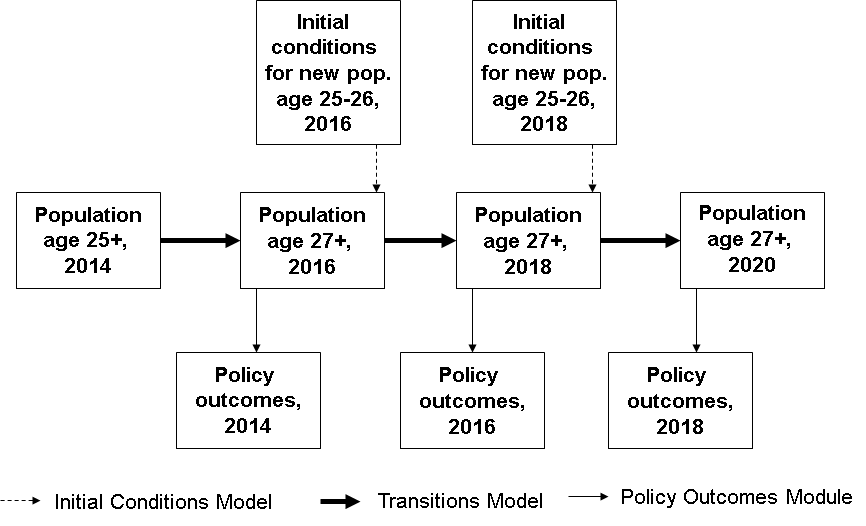
\includegraphics[scale=0.65]{./img/fam_architecture.png}
\caption{Architecture of the FAM}
\label{fig:fam_architecture} 
\end{figure}

Figure \ref{fig:fam_architecture} provides a schematic overview of the model. In this example, we start in 2014 with an initial population aged 25+ taken 
from the PSID. We then predict outcomes using our estimated transition probabilities (see section \ref{sec:estimation_transition_model}). Those who 
survive make it to the end of that year, at which point we calculate policy outcomes for the year. We then move 
to the following time period (two years later), when a replenishing cohort of 25 and 26 year-olds enters (see section 
\ref{sec:model_for_new_cohorts}). This entrance forms the new age 25+ population, which then proceeds through the transition model as before. This 
process is repeated until we reach the final year of the simulation. 
 
